\documentclass[11pt,a4paper]{jsarticle}
%
\usepackage{amsmath,amssymb}
\usepackage{bm}
\usepackage[dvipdfm]{graphicx}
\usepackage{ascmac}
\usepackage{float}
%
\setlength{\textwidth}{\fullwidth}
\setlength{\textheight}{39\baselineskip}
\addtolength{\textheight}{\topskip}
\setlength{\voffset}{-0.5in}
\setlength{\headsep}{0.3in}
%
\newcommand{\divergence}{\mathrm{div}\,}  %ダイバージェンス
\newcommand{\grad}{\mathrm{grad}\,}  %グラディエント
\newcommand{\rot}{\mathrm{rot}\,}  %ローテーション
%
\pagestyle{myheadings}
\markright{}
\begin{document}
%
%
\section*{用語補足資料}
\begin{itemize}
\item サルフェーション
\end{itemize}
\begin{flushleft}
極板に硫酸鉛の結晶が付着し、極板が化学反応しなくなる現象

開放型バッテリーの極板に白い結晶ができる現象であり、
このような状態になるとバッテリー液を補充しても元の状態に回復しなくなる

バッテリーを長期期間使用していると電極板に不活性な硫酸鉛が析出してくるため、バッテリーの通電機能の低下が起こる
\end{flushleft}

\begin{itemize}
\item LFC:Load Frequency Control(負荷周波数制御)
\end{itemize}
電力系統の負荷変動に対して、発電機出力を適切に制御調整し、各地域の周波数変動を許容値以内に収めること

\begin{itemize}
\item LFC調整容量
\end{itemize}
電力各社は、自系統内で発生する負荷変動をそれぞれの系統内で処理することを前提に、各社系統における固有の負荷変動の実態に応じて、必要な調整能力を調整容量と調整速度の両面から確保している

\begin{itemize}
\item 下げ代
\end{itemize}
計画的に出力を下げる方向の調整力

(総需要-ベース供給力-LFC調整力)

\begin{itemize}
\item ベース供給力
\end{itemize}
火力の最低出力,水力,原子力など

\begin{figure}[h]
\centering
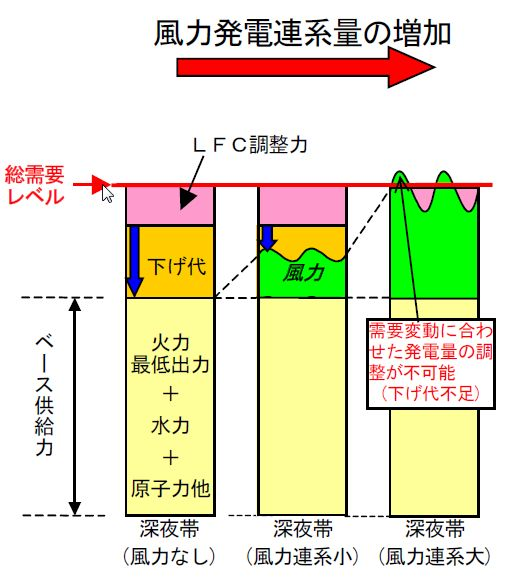
\includegraphics[width=6cm,bb=0 0 513 578]{WS000000.jpg}
\caption{風力が下げ代に与える影響}
\label{image_sample}
\end{figure}

%
%
\end{document}